\chapter{Transient resonances in extreme-mass-ratio inspirals}\label{ch:resonances}

\section{The general relativistic two-body problem}

In the prologue to his classic monograph, \citet{Chandrasekhar1992} celebrates the simplicity of BHs. The Kerr solution is defined by just two parameters: mass and spin. Despite the baldness of the BH metrics, great intricacies manifest in their properties. This is made evident when a second body is introduced. The two-body problem in GR is well studied. It is of paramount importance for GW astronomy, where binary systems are the dominant source of radiation. Correctly modelling the dynamics of these systems is necessary to interpret and extract information from gravitational waveforms.

\citet{Flanagan2012} highlighted a previously overlooked phenomenon that occurs in the general relativistic two-body problem, that of transient resonances. Geodesic orbits in GR have three associated frequencies: the radial frequency $\Omega_r$, the polar frequency $\Omega_\theta$ and the azimuthal frequency $\Omega_\phi$. The first two describe libration and the third rotation \citep[section 10.6]{Goldstein2002}.\footnote{There is an exception in the case of polar orbits, when $\Omega_\theta$ also describes rotation.} In the weak-field limit these all tend towards the Keplerian frequency and there is no orbital precession; in the strong-field $\Omega_r < \Omega_\theta < \Omega_\phi$, and they may differ significantly. For EMR systems, the evolution time-scale is much longer than the orbital period, such that the motion of the smaller body is approximately geodesic over orbital time-scales. The evolution of the orbit can be approximated as a series of geodesics using the osculating element formalism \citep{Pound2008,Gair2011a}. During the evolution the frequencies may become commensurate. Resonances occur when the radial and polar frequencies are rational multiples of each other:
\begin{equation}
\nu = \dfrac{\Omega_r}{\Omega_\theta} = \dfrac{n_\theta}{n_r},
\end{equation}
where $n_r$ and $n_\theta$ are integers (which we take to have no common factors). The azimuthal motion is not important because of the axisymmetry of the background spacetime. During resonance, terms in the self-force that usually average to zero can combine coherently, significantly impacting the motion \citep{Flanagan2012a}.

Geodesic motion in Kerr spacetime can be described by use of the action--angle formalism \citep[chapter 10]{Goldstein2002}. We consider a body of mass $\mu$ orbiting an MBH of mass $M_\bullet$, where $\eta = \mu/M_\bullet \ll 1$ and is used as a perturbative parameter, and describe the motion in the directions of the standard Boyer--Lindquist coordinates using generalised angle variables $q_\alpha = \{q_t,q_r,q_\theta,q_\phi\}$ \citep{Hinderer2008}. We denote the integrals of the geodesic motion, the generalised action variables, by $J_\alpha$. These are some combination of the energy per unit mass $E$, the axial angular momentum per unit mass $L_z$ and the Carter constant per unit mass squared $Q$ \citep{Carter1968}; we use $\mathcal{I}_a = \{E,L_z,Q\}$ for this set of three parameters. The system evolves following \citep{Flanagan2012}
\begin{subequations}\label{eq:Mino-E-o-M}
\begin{align}
\diff{q_\alpha}{\lambda} = {} & \omega_\alpha(\boldsymbol{J}) + \eta g_\alpha^{(1)}(q_r,q_\theta,\boldsymbol{J}) + \order{\eta^2}; \\
\diff{J_\alpha}{\lambda} = {} & \eta G_\alpha^{(1)}(q_r,q_\theta,\boldsymbol{J}) + \order{\eta^2},
\end{align}
\end{subequations}
where $\lambda$ is Mino time \citep{Mino2003}, and the forcing functions $g_\alpha^{(1)}$ and $G_\alpha^{(1)}$ originate from the first-order self-force. At zeroth order in the mass ratio we recover the limit of purely geodesic motion: the integrals of the motion are actually constants, and the angle variables evolve according to their associated frequencies $\omega_\alpha$.

The leading order dissipative correction to geodesic motion is calculated following the adiabatic prescription \citep{Hinderer2008}: by dropping the forcing term $g_\alpha^{(1)}$ (and all higher order terms) and replacing the forcing term $G_\alpha^{(1)}$ with its average over the $2$-torus parameterized by $q_r$ and $q_\theta$ $\langle G_\alpha^{(1)}\rangle_{q_r,\,q_\theta}$ \citep{Drasco2005}. For most orbits this is sufficient; $G_\alpha^{(1)}$ is given by its average value plus a rapidly oscillating component \citep[chapter 5, section 1]{Arnold1988}. However, this averaging fails when the ratio of frequencies is the ratio of integers. In this case the trajectory does not ergodically fill the $2$-torus but instead traces out a one-dimensional subspace.\footnote{For illustrations, see \citet{Grossman2012}.} There are then contributions to the self-force beyond $\langle G_\alpha^{(1)}\rangle_{q_r,\,q_\theta}$ that no longer average out over an orbit. Intuitively, we expect that this effect is more important for ratios of small integers, as when the integers are large the orbit comes close to all points on the $2$-torus.

In this chapter, we begin to characterise the importance of these resonances for the purposes of modelling EMRIs. We find the orbital parameters for which the orbital frequencies are commensurate (\secref{location}) and construct a formula to calculate the difference in the orbital parameters when comparing an adiabatic evolution with one that incorporates the instantaneous effects of the self-force (\secref{res-asymptotic}).

We use geometric units with $G = c = 1$ throughout. Hence the gravitational radius and its associate time-scale become $r\sub{g} = t\sub{g} = M_\bullet$.

\section{The theoretical framework of analysing resonances}

\subsection{Kerr geodesics}

The evolution of an extreme-mass-ratio ($\eta \ll 1$) system is slow. Instantaneously, the motion of the orbiting mass can be described as geodesic, with the integrals of the motion changing on time-scales of many orbital periods. We analyse the behaviour of resonances with the osculating element framework, where the trajectory is described by a sequence of geodesics which each match the position and velocity at a particular instance. It is therefore necessary to develop an understanding of the Kerr geodesics.\footnote{We have previously discussed motion in Kerr in \secref{Geodesic}.}

The geodesic equations are (\citealt{Carter1968}; \citealt[section 62]{Chandrasekhar1992})
\begin{subequations}
\begin{align}
\diff{t}{\lambda} = {} & a\left(L_z - aE\sin^2 \theta\right) + \dfrac{r^2 + a^2}{\Delta}\mathcal{T},\\
\diff{r}{\lambda} = {} & \pm \sqrt{V_r},\\
\diff{\theta}{\lambda} = {} & \pm \sqrt{V_\theta},\\
\diff{\phi}{\lambda}  = & \dfrac{L_z}{\sin^2 \theta} - aE + \dfrac{a}{\Delta}\mathcal{T},
\end{align}
\end{subequations}
where $\Delta = r^2 - 2M_\bullet r + a^2$; the signs of the $r$ and $\theta$ equations may be chosen independently, and we have used
\begin{subequations}
\begin{align}
\mathcal{T} = {} & E\left(r^2 +a^2\right) - aL_z,\\
V_r = {} & \mathcal{T}^2 - \Delta\left[r^2 + \left(L_z -aE\right)^2 + Q\right],\\
V_\theta = {} & Q - \cos^2 \theta\left[a^2\left(1 - E^2\right) + \dfrac{L_z^2}{\sin^2\theta}\right].
\end{align}
\end{subequations}
As an affine parameter we have used Mino time, which is related to the proper time $\tau$ by \citep{Mino2003}
\begin{equation}
\tau = \intd{}{}{r^2 + a^2 \cos^2\theta}{\lambda}.
\end{equation}
Using Mino time allows us to decouple the $r$ and $\theta$ motions.

We only consider bound motion \citep{Wilkins1972}. The radial motion covers a range $r\sub{p} \leq r \leq r\sub{a}$ where the turning points are the periapsis $r\sub{p}$ and apoapsis $r\sub{a}$. Drawing upon Keplerian orbits we parameterize the motion using
\begin{equation}
r = \dfrac{p}{1+e\cos\psi},
\end{equation}
with eccentricity $e$; semilatus rectum $p$, and relativistic anomaly $\psi$, which increases secularly by $2\pi$ over an orbit  \citep{Darwin1961,Drasco2004}. The polar motion covers a range $\theta_- \leq \theta \leq \pi - \theta_-$. We parameterize this motion in terms of $\chi$ according to \citep{Hughes2000}
\begin{equation}
\cos\theta = \cos\theta_-\cos\chi.
\end{equation}
Whilst $\psi$ and $\chi$ are $2\pi$ periodic, they are not the canonical action--angle variables \citep{Schmidt2002}; they are, however, easy to work with.

The geodesic motion can equally be described by $\{E,L_z,Q\}$ or $\{p,e,\theta_-\}$ \citep{Schmidt2002}. Converting between them requires finding the solutions of $V_r = 0$ and $V_\theta = 0$. We employ a slightly different parameter set of $\{p,e,\iota\}$ with inclination defined by \citep{Ryan1996,Glampedakis2002}
\begin{equation}
\tan \iota = \dfrac{\sqrt{Q}}{L_z}.
\end{equation}
With this definition, $0 \leq \iota < \pi/2$ for pro grade orbits and $\pi/2 < \iota \leq \pi$ for retrograde orbits. Equatorial orbits ($\theta_- = \pi/2$) have $\iota = 0$ or $\pi$ and polar orbits ($\theta_- = 0$) have $\iota = \pi/2$. Whilst formulae exist for conversion between the different parameters, they are complicated and uninsightful, so we do not reproduce them here.\footnote{In practice we find turning points numerically.}

\subsection{Orbital resonances}

The radial and polar orbital periods in Mino time are given by
\begin{subequations}
\begin{align}
\Lambda_r = {} & 2\intd{r\sub{p}}{r\sub{a}}{\recip{\sqrt{V_r}}}{r} = \intd{-\pi}{\pi}{\diff{\lambda}{\psi}}{\psi}, \\
\Lambda_\theta = {} & 4\intd{\theta_-}{\pi/2}{\recip{\sqrt{V_\theta}}}{\theta} = \intd{-\pi}{\pi}{\diff{\lambda}{\chi}}{\chi}.
\end{align}
\end{subequations}
The orbital frequencies are thus
\begin{equation}
\Upsilon_r = \dfrac{2\pi}{\Lambda_r}, \quad \Upsilon_\theta = \dfrac{2\pi}{\Lambda_\theta}.
\end{equation}
The geodesic equations for coordinate time $t$ and azimuthal angle $\phi$ are just functions of $r$ and $\theta$, hence their evolutions can be expressed as Fourier series \citep{Drasco2004}
\begin{subequations}
\begin{align}
\diff{t}{\lambda} = {} & \sum_{k_r,\,k_\theta}T_{k_r,\, k_\theta}\exp\left[-i\left(k_r\Upsilon_r + k_\theta\Upsilon_\theta\right)\lambda\right], \\
\diff{\phi}{\lambda} = {} & \sum_{k_r,\,k_\theta}\Phi_{k_r,\, k_\theta}\exp\left[-i\left(k_r\Upsilon_r + k_\theta\Upsilon_\theta\right)\lambda\right].
\end{align}
\label{eq:Mino-Fourier}
\end{subequations}
The $(0,\,0)$ coefficients in these series give the average secular rate of increase of these quantities. We define
\begin{equation}
\Gamma = T_{0,\,0}, \quad \Upsilon_\phi = \Phi_{0,\,0}
\end{equation}
as the Mino time frequencies. We can now convert to coordinate time frequencies with
\begin{equation}
\Omega_r = \dfrac{\Upsilon_r}{\Gamma}, \quad \Omega_\theta = \dfrac{\Upsilon_\theta}{\Gamma}, \quad \Omega_\phi = \dfrac{\Upsilon_\phi}{\Gamma}.
\end{equation}

Transient resonances occur when the radial and polar motions are commensurate, when
\begin{equation}
\nu = \dfrac{\Upsilon_r}{\Upsilon_\theta} = \dfrac{\Omega_r}{\Omega_\theta} = \dfrac{n_\theta}{n_r}
\end{equation}
is the ratio of (small) integers. At this point any Fourier series, like those in \eqnref{Mino-Fourier}, goes from being an expansion in two frequencies to being an expansion in a single frequency \citep{Bosley1992}.

On resonance, the radial and polar motions are locked together such that we can express one as a function of the other. For a general non-resonant orbit there is no fixed correlation between two coordinates. After a sufficiently long time, the trajectory comes arbitrarily close to every point in the range of motion (with $r\sub{p} \leq r \leq r\sub{a}$ and $\theta_- \leq \theta \leq \pi - \theta_-$); on account of the orbital precession, the whole space is densely covered. This does not happen on resonance as the trajectory keeps cycling over the same path. The points visited are controlled by the relative phases of the $r$ and $\theta$ motions. To characterise this, we use the $\theta$ phase at periapsis $\chi\sub{p}$; Varying $\chi\sub{p}$ across its full range allows every point in the range of motion to be reached. Hence averaging over all values of $\chi\sub{p}$ for a resonant orbit is equivalent to averaging over the $\psi$--$\chi$ $2$-torus for non-resonant orbits.

One might be concerned about the nature of resonances following the inclusion of the self-force: true geodesic motion only exists at zeroth order in $\eta$ and, whilst it is a good approximation over short time-scales, for small $\eta$ there is a small disparity. The conservative piece of the self-force induces extra precession which leads to a slight shift in the orbital frequencies \citep{Warburton2012}.\footnote{The Kolmogorov--Arnold--Moser (KAM) theorem states that when an integrable Hamiltonian (i.e., the case for motion in Kerr) is subject to a small perturbation the form of the orbits is preserved albeit slightly deformed (\citealt{Arnold1963}; \citealt[chapter II, section 3.3 d]{Moser1973}). This should ensure that, in general, there are only small shifts in the orbital frequencies. However, the KAM theory only applies for sufficiently incommensurate orbits: close to resonance it does not apply \citep[chapter V, section 1 c]{Moser1973}. This is a further reason why resonances merit an in-depth investigation.} The dissipative piece causes the frequencies to evolve and, hence, the resonance cannot persist for multiple orbits (without some feedback coupling). In effect, we are really considering a period of time about the resonant crossing. The instantaneous orbital frequencies oscillate back and forth around their averaged values; a generic example of this behaviour is shown in \figref{wibbles}.
\begin{figure}%[tbhp]
\centering
\vspace{0.25\baselineskip}
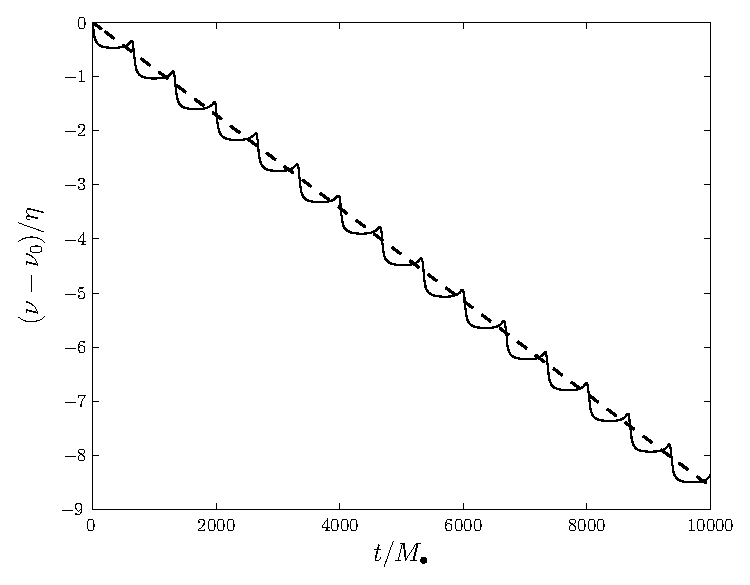
\includegraphics[width=0.6\textwidth]{./images/Fig_ad_vs_inst_wibble}
\caption{Evolution of the frequency ratio $\nu$ under both adiabatic (dashed line) and instantaneous evolutions (solid line). The two coincide at $t = 0$ when $\nu = \nu_0$. The behaviour is general, cf.\ figure 27 of \citet{Arnold1988}. In this particular example, $\nu_0 \simeq 0.685$, $\eta = 10^{-6}$ and $a_\ast = 0.9$, the initial orbital parameters are $p = 10 M_\bullet$, $e = 0.7$ and $\cos \iota = 0.2$; there are no significant resonances in the plotted span. As a reference for the time-span, the azimuthal orbital period is $T_\phi \simeq 432 M_\bullet$. Data courtesy of Robert Cole.}\label{fig:wibbles}
\end{figure}
However, there shall be a time span when the frequencies are consistently close to being commensurate. During this time the trajectory appears similar to a resonant trajectory, filling only a smaller region of the parameter space. It is this time period that is of interest for transient resonances \citep{Bosley1992}.

%\subsection{Self-force model}

%To follow the evolution of the inspiral we must have a means of modelling the self-force. In this work we use the same post-Newtonian approximation as \citet{Flanagan2012}. They use the first-order post-Newtonian terms of the dissipative self-force formulated in Flanagan and Hinderer \citep{Flanagan2007} and the conservative force formulated in \citet{Iyer1993}, and \citet{Kidder1995}. Since only the first post-Newtonian terms are used, this prescription can only be of limited validity in strong fields. Both pieces of the self-force are computed assuming that the spin is small: the dissipative piece contains terms to $\order{a_\ast^2}$ and the conservative piece to $\order{a_\ast}$. This is less than ideal for high spins. While this approximate self-force is not perfect, it should serve as a guide for the behaviour of the full self-force.

%For comparison, Flanagan, Hughes and Ruangeri \citep{Flanagan2012a} use a Teukolsky equation calculation of GW fluxes to account for radiation reaction.

\section{Location of resonances}\label{sec:location}

The first step in studying the effect of transient resonance is to locate orbital parameters for which the frequencies are commensurate. We can calculate the frequencies, and so we are left with the problem of solving $\Omega = n_r \Omega_r - n_\theta \Omega_\theta = 0$ numerically. \Figref{res-plane-2-5-95} shows the semilatus rectum, eccentricity and (cosine of the) inclination angle of the $\nu = 2/5$ resonance surface for an MBH of spin $a_\ast = 0.95$. 
\begin{figure}%[htbp]
\centering
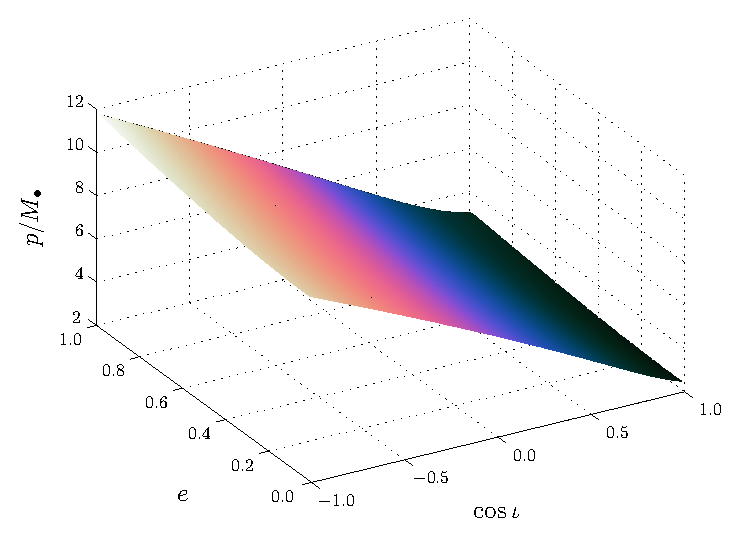
\includegraphics[width=0.6\textwidth]{./images/Fig_res-2-5-95-plane}
\caption{Location of the $2/5$ resonance surface for an $a_\ast = 0.95$ MBH in terms of orbital semilatus rectum $p$, eccentricity $e$ and inclination $\iota$. Data courtesy of Robert Cole.}\label{fig:res-plane-2-5-95}
\end{figure}
The resonances occur at relatively small periapses, corresponding to regions of strong-field gravity.
Similar resonance surfaces can be found for other spin values and for other resonances. When considering the full parameter set of $\{p,e,\iota,a_\ast,\nu\}$ it is apparent that the search for resonances becomes expensive as a consequence of the dimensionality. It is therefore useful to have a guide of where to look. We shall attempt to build a model for the resonance plane.

\citet{Brink2013} provide series expansions for the location of resonances in the limit of equatorial orbits for small spin and eccentricity. We do not follow this approach of trying to find analytic expressions for the resonance surface. The expressions become complicated when venturing away from limiting cases. Instead, we build an approximate phenomenological model and fit this to the resonance plane. %\footnote{A stopped clock is precisely correct twice a day, while a clock that is five minutes slow is never right but will often be close enough. Within this metaphor, our approximation would be a clock that varies between telling the correct time and being fifteen minutes off throughout the day: it is generally going to be good enough to give you a sense of the time but if you have an important event you should check with something better.}
This should be useful for designating the region in which resonance could be expected. To locate resonances precisely it is necessary to solve $\Omega = 0$ numerically; the approximate model should give a suitable starting point.

The resonant semilatus rectum for any particular spin and resonance ratio can be well approximated as
\begin{equation}
p(e,\iota;a_\ast,\nu) \simeq A\dfrac{1 + B e + D \cos\iota}{1 - C\exp(e)} M_\bullet.
\end{equation}
The coefficients $\{A,B,C,D\}$ depend upon the spin and the particular resonance; they can be approximated as
\begin{align} 
A(a_\ast,\nu) \simeq {} & a_0\dfrac{1 + a_1\nu - a_2 \nu^2 - a_3 \nu a_\ast^2}{1 + a_4\nu - (1 + a_4)\nu^2}, \\
B(a_\ast,\nu) \simeq {} & b_0(1 - b_1\nu)\exp(-b_2\nu)(1 - b_3 a_\ast), \\
C(a_\ast,\nu) \simeq {} & c_0, \\
D(a_\ast,\nu) \simeq {} & d_0\left[1 - \exp(a_\ast)\right]\left[1 - d_1\exp(\nu)\right].
\end{align}
This gives us a total of $12$ parameters for our fit. While this may sound large, if we were fitting an expansion to quadratic order in any combination of $\{e,\iota,a_\ast,\nu\}$ we would have $15$ parameters.\footnote{This does not give as good a fit as our function.} Our best fit parameters are
\begin{equation}
\begin{array}{c}
a_0 = 5.9854; \quad a_1 = 3.4116; \quad a_2 = 0.9253; \quad a_3 = 0.1959; \\
a_4 = 4.8846; \quad b_0 = 0.7692; \quad b_1 = 1.4752; \quad b_2 = 1.4861; \\
b_3 = 0.5974; \quad c_0 = 0.02332; \quad d_0 = 0.7968; \quad d_1 = 0.3115.\end{array}
\end{equation} 
These were fitted for resonances with $\nu = 1/7$, $1/6$, $1/5$, $1/4$, $2/7$, $1/3$, $2/5$, $3/7$, $1/2$, $4/7$, $3/5$, $2/3$, $5/7$, $3/4$, $4/5$, $5/6$, $6/7$, $9/10$, $19/20$, $49/50$ and $99/100$; with MBH spins of $a_\ast = 0.01$, $0.05$, $0.1$, $0.2$, $0.3$, $0.4$, $0.5$, $0.6$, $0.7$, $0.8$, $0.9$, $0.93$, $0.95$, $0.97$, $0.99$ and $0.999$; for orbits with eccentricities $0.01 \leq e \leq 0.99$, and inclinations $-0.999999 \leq \cos\iota \leq 0.999999$. Using our approximation, the maximum error in $p$ for a given $a_\ast$ and $\nu$ is typically $\sim10\%$ and less that $1 M_\bullet$ in absolute terms. The relative error in the semilatus rectum is illustrated in \figref{p-error}. 
\begin{figure}%[htp]
\centering
 \subfigure[{Maximum error}]{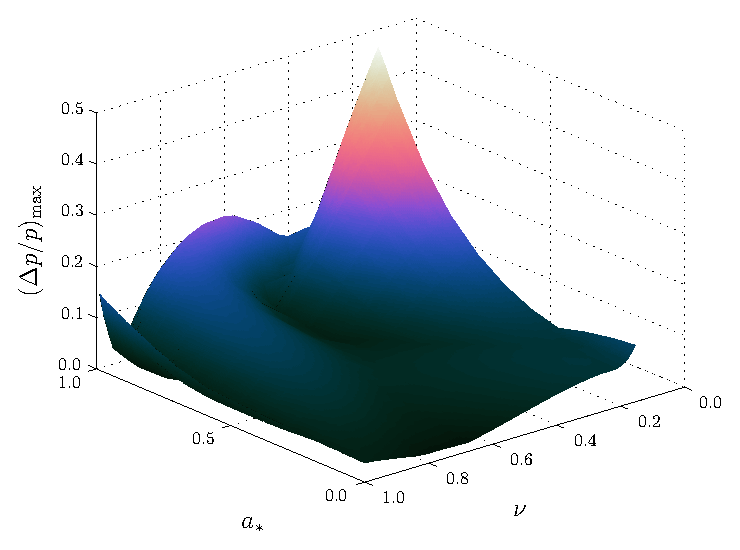
\includegraphics[width=0.475\textwidth]{./images/Fig_fit-error-max-plane}} \quad \subfigure[{Root-mean-square error}]{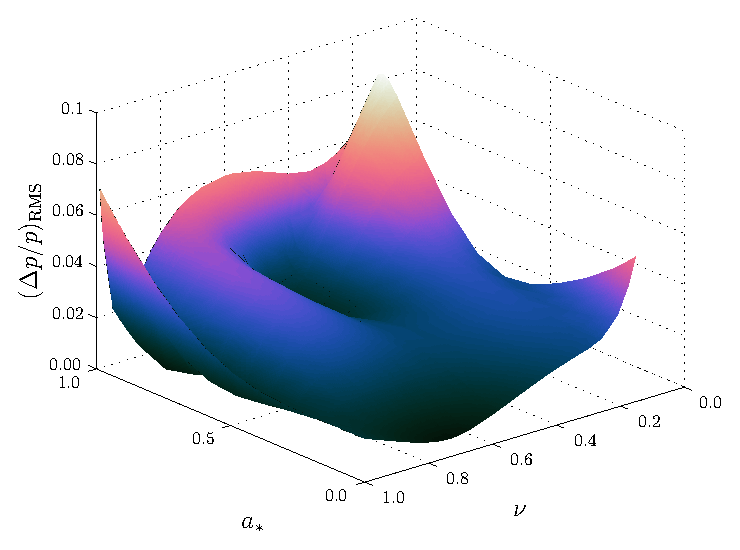
\includegraphics[width=0.475\textwidth]{./images/Fig_fit-error-RMS-plane}}
\caption{Relative error in the approximate semilatus rectum compared to the accurate numerical result as a function of MBH spin $a_\ast$ and resonance ratio $\nu$. In both figures we are marginalising over eccentricity and inclination.}\label{fig:p-error}
\end{figure}
The largest fractional error is $\sim50\%$, this is for $a_\ast \rightarrow 1$ and $\nu \rightarrow 0$, and corresponds to small $p/M_\bullet$, such that the absolute error is still small. Taking the root-mean-square across $e$ and $\iota$, the fractional error for a given $a_\ast$ and $\nu$ never exceeds $9\%$ and is typically less than $4\%$.

\section{Importance of resonances}\label{sec:importance}

Having determined the location of resonances, we may now address their importance. We wish to quantify the enhancement (or decrement) of the flux of $E$, $L_z$ and $Q$ during resonance and, equivalently, the change in $p$, $e$ and $\iota$. A change in the orbital parameters relative to the adiabatic prescription leads to a dephasing of waveforms. This is of interest for a matched filtering analysis of inspirals.

\subsection{Time-scales}\label{sec:res-time}

When analysing resonances it is useful to refer to a number of reference time-scales. We always use coordinate time $t$ for these, as this corresponding to what is measured by an observer at infinity. Translation to Mino time can be done with an appropriate factor of $\Gamma$. We use the orbital period $T$, the evolution time-scale $\tau\sub{ev}$, the precession time-scale $\tau\sub{pres}$ and the resonance time-scale $\tau\sub{res}$.

The simplest time-scales are the orbital periods $T_r = 2\pi/\Omega_r$, $T_\theta = 2\pi/\Omega_\theta$ and $T_\phi = 2\pi/\Omega_\phi$. These are the shortest in our set. We use $T$ to denote a time-scale of the same order as the orbital periods.

We define the evolution time-scale as
\begin{equation}
\tau\sub{ev} = \dfrac{\nu}{\dot{\nu}},
\end{equation}
where an overdot denotes a derivative with respect to $t$. In general, away from resonance, we take $\nu \equiv \Omega_r/\Omega_\theta$. This time-scale sets the period over which there is a significant change in the frequencies. It represents the inspiral time-scale. It is long in all cases we study, $\tau\sub{ev} \sim \order{\eta^{-1}T}$. It is this property which makes EMRIs interesting, as we can follow the waveform for many cycles, accruing high SNRs. This is also what allows us to use the adiabatic prescription, as it means that the trajectory moves slowly through different orbital parameters.

We use the precession time-scale
\begin{equation}
\tau\sub{pres}(t) = \dfrac{2\pi}{|\Omega(t)|},
\label{eq:t-pres}
\end{equation}
with $\Omega(t) = n_r \Omega_r(t) - n_\theta \Omega_\theta(t)$, where the frequencies are calculated instantaneously, and the integers are for the resonance of interest. This time-scale becomes infinite exactly on resonance, but decreases as we get further from resonance. It measures the relative precession rate of the radial and polar motions, and hence gives an indication of how long it takes to fill the entire $\psi$--$\chi$ $2$-torus.

We also use the resonance time-scale
\begin{equation}
\tau\sub{res} = \left[\dfrac{2\pi}{\left|\langle\dot{\Omega}(0)\rangle_{q'}\right|}\right]^{1/2}.
\label{eq:t-res}
\end{equation}
Here $\dot{\Omega}(0)$ is the rate of change of $\Omega$ at resonance, which we take to be at $t = 0$. The instantaneous $\dot{\Omega}$ depends upon the orbital phase and oscillates about its mean trend over an orbit (see \figref{wibbles}). We are interested in the averaged behaviour, not the periodic modulations about this, which is why we use the phase-averaged trend $\langle\dot{\Omega}\rangle_{q'}$.\footnote{Here we use $q'$ to represent a phase that varies over an orbit with period $T$; it is introduced again in \secref{res-asymptotic}.} Close to resonance, $\Omega$ is well approximated by a first-order Taylor expansion, decreasing linearly with time; hence we make the approximation
\begin{equation}
\left|\langle\dot{\Omega}\rangle_{q'}\right| \simeq \left|\dfrac{\Omega(t)}{t}\right|.
\end{equation}
The resonant time-scale should give an indication of the time over which we expect the effects of the resonance to be felt \citep{Bosley1992}. If we consider the phase of the Mino time Fourier expansion on resonance, neglecting the constant, the resonant Fourier component has form
\begin{equation}
\varphi_{n_r,\,-n_\theta} \simeq \left(n_r\Upsilon_r - n_\theta\Upsilon_\theta\right)\lambda + \left(n_r\dot{\Upsilon}_r - n_\theta\dot{\Upsilon}_\theta\right)\lambda^2 + \ldots
\end{equation}
Typically, the first term is non-zero and this gives the familiar oscillation. On resonance it is zero, leaving the next order term to govern the behaviour \citep{Flanagan2012}. Only once we have moved far enough away from resonance for the first term to dominate the second do we recapture the non-resonant behaviour. The first term (translating from Mino time to coordinate time) sets $T$, the second sets $\tau\sub{res}$.

Since we have argued that the effect of resonance can be thought of as a consequence of not densely covering the $\psi$--$\chi$ $2$-torus, we might expect that $\tau\sub{pres}$, as well as $\tau\sub{res}$, could be used for setting the resonance duration: the resonance ends once sufficient time has elapsed that the $2$-torus could be filled. This is indeed the case. Let $t\sub{pres}$ be the time taken to fill the torus, then
\begin{align}
t\sub{pres} = {} & \tau\sub{pres}(t\sub{pres}) \\
 \simeq {} & \dfrac{2\pi}{\left|\langle\dot{\Omega}(0)\rangle_{q'} t\sub{pres}\right|}, \nonumber 
\end{align}
using \eqnref{t-pres} and substituting $\Omega(t\sub{pres}) \simeq \langle\dot{\Omega}(0)\rangle_{q'} t\sub{pres}$. Rearranging and using \eqnref{t-res} gives
\begin{equation}
t\sub{pres} \simeq \tau\sub{res}.
\end{equation}
The two time-scales are equivalent. We shall preferentially use $\tau\sub{res}$ to denote the resonance width. It is shorter than the inspiral time-scale, but longer than an orbital period, $\tau\sub{res} \sim \order{\eta^{1/2}\tau\sub{ev}} \sim \order{\eta^{-1/2}T}$ \citep{Flanagan2012,Gair2011a}; it therefore acts as a bridge between the two time-scales \citep{Hinderer2008}.

Since we shall be considering Fourier decompositions, in anticipation of future results, we also define a time-scale for the $s$-th resonant frequency harmonic
\begin{align}
%\tau_{\mathrm{pres},\,s} = {} & \dfrac{2\pi}{|s\Omega(t)|};\\
\tau_{\mathrm{res},\,s} = {} & \left[\dfrac{2\pi}{\left|\langle s\dot{\Omega}(0)\rangle_{q'}\right|}\right]^{1/2}.
\label{eq:T-res-s}
\end{align}
This assumes that $s$ is a non-zero integer.

\subsection{Asymptotic solution for passage through resonance}\label{sec:res-asymptotic}

The impact of passing through resonance on the evolution can be modelled analytically using asymptotic expansions \citep{Gair2012}. Solutions for the motion are constructed far away from resonance and these are matched to a transition region in the vicinity of resonance \citep{Kevorkian1971,Bosley1992}. By comparing the matched solution, which incorporates the effects of resonance, with the results of an adiabatic evolution, it is possible to estimate the discrepancy in the orbital parameters. This determines the difference in the orbital phase between the two approaches. If this error is sufficiently small, then it is safe to ignore the effects of the resonance; however, only a small difference is needed to impact the subsequent waveform, since the error accumulates over the subsequent observation of $\sim \order{\eta^{-1}}$ cycles \citep{Flanagan2012}. We derive formulae which can be used to calculate the discrepancy in the orbital parameters.

The following derivation is based upon the analysis of \citet{Kevorkian1987}.\footnote{The same theory underpins the analysis of \citet{Hinderer2008}, but this explicitly ignores resonances.} Small adjustments have been made to adapt to the specific problem of GW inspiral, but the general argument is unchanged.

We model the system using action--angle variables. We are only concerned with the $r$ and $\theta$ motions, so we have a two-dimensional system. We perform a canonical transformation  to isolate the resonant combination $q = n_r q_r - n_\theta q_\theta$ \citep{Bosley1992}. This becomes one of the new angle variables, the other variable $q'$ can be either $q_r$ or $q_\theta$ (as, on resonance, varying one necessarily changes the other). We use $J$ as the conjugate action variable to $q$ and $\omega = n_r \omega_r - n_\theta \omega_\theta$ as its frequency. Similarly, we use $J'$ as the action variable conjugate to $q'$. The system evolves through resonance slowly, on an evolution time-scale, so we parameterize it in terms of a slow time parameter
\begin{equation}
\widetilde{\lambda} = \eta\lambda.
\end{equation}
The orbits of $q'$ proceed with the fast time $\lambda$; since this is much more rapid than the evolution we are interested in, it is safe to average over it. We are not interested in the fine-grained fast oscillations caused by changes in $q'$. For this analysis we consider the reduced problem of evolving $q$ and $J$.

At resonance $\widetilde{\lambda} = \widetilde{\lambda}_\star$ and $\omega\left(\widetilde{\lambda}_\star\right) = 0$. We assume that the frequency has a simple zero and can be expanded as
\begin{equation}
\omega\left(\widetilde{\lambda}\right) = \varpi_1\left(\widetilde{\lambda} - \widetilde{\lambda}_\star\right) + \varpi_2\left(\widetilde{\lambda} - \widetilde{\lambda}_\star\right)^2 + \ldots
\label{eq:omega-series}
\end{equation}
The frequency is actually a function of the angle variables, but since these evolve with $\widetilde{\lambda}$ it is safe to write it as a function of the slow time.\footnote{In effect we are defining $\omega\left(\widetilde{\lambda}\right) \equiv \omega\left[J\left(\widetilde{\lambda}\right)\right]$.}

Using the slow time, the equations of motion (\ref{eq:Mino-E-o-M}) become
\begin{subequations}
\begin{align}
\diff{q}{\widetilde{\lambda}} = {} & \dfrac{\omega(J)}{\eta} + \sum_s g_s^{(1)}(J)\exp(is q)  + \order{\eta}; \\
\diff{J}{\widetilde{\lambda}} = {} & \sum_s G_s^{(1)}(J)\exp(is q) + \order{\eta},
\end{align}
\end{subequations}
where we have rewritten the forcing terms as Fourier series and adapted the forcing functions to those appropriate for $q$ and $J$. We shall solve these before resonance and then match these to a solution in the transition regime about resonance.

\subsubsection{Solution before resonance}\label{sec:before-res}

To find a solution away from the resonance, we decompose the problem to be a function of two time-scales \citep{Kevorkian1971}. We use the slow time $\widetilde{\lambda}$ and, as a proxy for the fast time,
\begin{equation}
\Psi = \intd{0}{\lambda}{\omega(\eta\tau)}{\tau} = \recip{\eta}\intd{0}{\tilde{\lambda}}{\omega(\widetilde{\tau})}{\widetilde{\tau}}.
\end{equation}
From this
\begin{equation}
\omega = \diff{\Psi}{\lambda}.
\end{equation}
In terms of these two variables, we can build ansatz solutions
\begin{subequations}
\begin{align}
\label{eq:q-series}
q(\lambda;\,\eta) = {} & \Psi + q_0\left(\widetilde{\lambda}\right) + \eta q_1\left(\Psi,\widetilde{\lambda}\right) + \order{\eta^2}; \\
J(\lambda;\,\eta) = {} & J_0\left(\widetilde{\lambda}\right) + \eta J_1\left(\Psi,\widetilde{\lambda}\right) + \order{\eta^2}.
\label{eq:J-series}
\end{align}
\end{subequations}
We can also write a series expansion for the frequency, since it is affected by the self-force too,
\begin{equation}
\omega(\lambda;\,\eta) = \omega_0\left(\widetilde{\lambda}\right) + \eta \omega_1\left(\widetilde{\lambda}\right) + \order{\eta^2}.
\end{equation}
In the limit of $\eta \rightarrow 0$ we are left with a constant frequency $\omega_0(0)$. The higher order terms are identified below by matching terms in the series expansion of the equations of motion. Taking the two time-scales as independent, we may write the time derivative to $\order{\eta}$ as
\begin{equation}
\diffop{\lambda} = \omega_0\partialdiffop{\Psi} + \eta\omega_1\partialdiffop{\Psi} + \eta\partialdiffop{\widetilde{\lambda}}.
\end{equation}

Using the two time-scale decomposition to replace the time derivatives in the equations of motion, and substituting in the ansatz expansions gives, to first order,
\begin{subequations}
\begin{align}
\label{eq:q-1}
\omega_0 + \eta\omega_1 + \eta\partialdiff{q_0}{\widetilde{\lambda}} + \eta\omega_0\partialdiff{q_1}{\Psi} = {} & \omega(J_0) + \eta\diff{\omega}{J}J_1 + \eta \sum_s g_s^{(1)}(J_0)\exp(is \Psi + Q_0); \\
\eta\partialdiff{J_0}{\widetilde{\lambda}} + \eta\omega_0\partialdiff{J_1}{\Psi} = {} & \eta \sum_s G_s^{(1)}(J_0)\exp(is \Psi + Q_0).
\label{eq:J-1}
\end{align}
\end{subequations}
Averaging \eqnref{J-1} over $\Psi$ gives\footnote{The ansatz is constructed such that $J_0 \equiv \langle J_0\rangle_\Psi$ and $q_0 \equiv \langle q_0\rangle_\Psi$.}
\begin{equation}
\partialdiff{J_0}{\widetilde{\lambda}} = G_0^{(1)}(J_0).
\label{eq:J-ad}
\end{equation}
This describes the adiabatic evolution, hence we can identify $J_0\left(\widetilde{\lambda}\right)$ with (the lowest order piece of) the adiabatic solution \citep{Hinderer2008}. If we similarly average \eqnref{q-1} we find
\begin{equation}
\omega_0 + \eta\omega_1 +\eta\partialdiff{q_0}{\widetilde{\lambda}} = \omega(J_0) + \eta\partialdiff{\omega}{J}\langle J_1\rangle_\Psi + \eta g_0^{(1)}(J_0).
\end{equation}
From this we can identify the terms that originate from the frequency and, matching by order in $\eta$, obtain
\begin{subequations}
\begin{align}
\omega_0 = {} & \omega(J_0); \\
\omega_1 = {} & \partialdiff{\omega}{J}\langle J_1\rangle_\Psi.
\end{align}
\end{subequations}
This leaves
\begin{align}
\partialdiff{q_0}{\widetilde{\lambda}} = {} & g_0^{(1)}(J_0); \\
q_0 = {} & \kappa_0 + \intd{0}{\tilde{\lambda}}{g_0^{(1)}[J_0(\tau)]}{\tau}.
\label{eq:q-0-sol}
\end{align}
We now have expressions for the lowest order terms in the expansions.

Subtracting the $s = 0$ components from \eqnref{J-1} leaves
\begin{equation}
\omega_0\partialdiff{J_1}{\Psi} = \sum_{s\,\neq\,0} G_s^{(1)}(J_0)\exp(is \Psi + Q_0).
\end{equation}
This can be solved to give
\begin{equation}
J_1 = \langle J_1\rangle_\Psi + \recip{\omega_0}\sum_{s\,\neq\,0} \dfrac{G_s^{(1)}(J_0)\exp(is \Psi + Q_0)}{is}.
\label{eq:J-1-sol}
\end{equation}
We can do the same for \eqnref{q-1} to obtain
\begin{equation}
q_1 = \langle q_1\rangle_\Psi + \recip{\omega_0}\sum_{s\,\neq\,0} \dfrac{g_s^{(1)}(J_0)\exp(is \Psi + Q_0)}{is}.
\label{eq:q-1-sol}
\end{equation}
To find the constants of integration, $\langle q_1\rangle_\Psi$ and $\langle J_1\rangle_\Psi$, it is necessary to extend the analysis to second order in $\eta$. This shows that $\langle J_1\rangle_\Psi$ is the first-order component of the adiabatic solution. We do not need explicit forms for later calculations, so we will not proceed further. We have successfully constructed the pre-resonance solution.

\subsubsection{Solution near resonance}\label{sec:interior-res}

Near to resonance, we consider an interior layer expansion \citep{Kevorkian1971}. As explained in \secref{res-time}, evolution near resonance proceeds on a time-scale intermediate between the slow and fast times. We therefore introduce a rescaled time
\begin{equation}
\widehat{\lambda} = \dfrac{\widetilde{\lambda} - \widetilde{\lambda}_\star}{\eta^{1/2}} = \eta^{1/2}(\lambda - \lambda_\star).
\end{equation}
As for the before resonance solution, we can create a series expansion; however, now we expand in terms of $\eta^{1/2}$ \citep{Flanagan2012}
\begin{subequations}
\begin{align}
q\left(\widehat{\lambda};\,\eta\right) = {} & \widehat{q}_0\left(\widehat{\lambda}\right) + \eta^{1/2} \widehat{q}_{1/2}\left(\widehat{\lambda}\right) + \order{\eta}; \\
J\left(\widehat{\lambda};\,\eta\right) = {} & \widehat{J}_0 + \eta^{1/2} \widehat{J}_1\left(\widehat{\lambda}\right) + \order{\eta}.
\end{align}
\end{subequations}
The series expansion for the frequency, \eqnref{omega-series}, can be rewritten as
\begin{equation}
\omega\left(\widehat{\lambda}\right) = \eta^{1/2}\varpi_1\widehat{\lambda} + \eta\varpi_2\widehat{\lambda}^2 + \order{\eta^{3/2}}.
\label{eq:omega-hat}
\end{equation}
Proceeding to write the equations of motion in terms of the rescaled time gives
\begin{subequations}
\begin{align}
\diff{q}{\widehat{\lambda}} = {} & \varpi_1\widehat{\lambda} + \eta^{1/2}\varpi_2\widehat{\lambda}^2 + \eta^{1/2}\sum_s g_s^{(1)}\left(\widehat{J}_0,\widetilde{\lambda}_\star\right)\exp(is \widehat{q}_0)  + \order{\eta}; \\
\diff{J}{\widehat{\lambda}} = {} & \eta^{1/2}\sum_s G_s^{(1)}\left(\widehat{J}_0,\widetilde{\lambda}_\star\right)\exp(is \widehat{q}_0) + \order{\eta}.
\end{align}
\end{subequations}

From the equations of motion we can match terms by their order in $\eta^{1/2}$. At zeroth order we find
\begin{equation}
\widehat{J}_0 = \widehat{\varrho}_0
\end{equation}
is constant, and
\begin{equation}
\widehat{q}_0 = \widehat{\kappa}_0 + \dfrac{\varpi_1\widehat{\lambda}^2}{2}.
\end{equation}
Using these, we can build the next order terms
\begin{align}
\widehat{q}_{1/2} = {} & \widehat{\kappa}_{1/2} + \dfrac{\varpi_2\widehat{\lambda}^3}{3} + g_0^{(1)}(\widehat{\varrho}_0)\widehat{\lambda} + \sum_{s\,\neq\,0}g_s^{(1)}(\widehat{\varrho}_0)\exp(is \widehat{\kappa}_0)\intd{0}{\hat{\lambda}}{\exp\left(\dfrac{is \varpi_1\tau^2}{2}\right)}{\tau}; \\
\widehat{J}_{1/2} = {} & \widehat{\varrho}_{1/2} + G_0^{(1)}(\widehat{\varrho}_0)\widehat{\lambda} + \sum_{s\,\neq\,0}G_s^{(1)}(\widehat{\varrho}_0)\exp(is \widehat{\kappa}_0)\intd{0}{\hat{\lambda}}{\exp\left(\dfrac{is \varpi_1\tau^2}{2}\right)}{\tau}.
\end{align}
Both of these involve the complex Fresnel integral \citep[chapter 7]{Olver2010}, the details of which are given in the following section. We have now constructed the interior solution.

\subsubsection{The complex Fresnel integral}

The solution for the motion in the interior region near to resonance involves the integral
\begin{equation}
W\left(\widehat{\lambda}\right) = \intd{0}{\hat{\lambda}}{\exp\left(\dfrac{is \varpi_1\tau^2}{2}\right)}{\tau}.
\end{equation}
The complex Fresnel integral is
\begin{equation}
\mathcal{Y}(z) = \intd{0}{z}{\exp\left(\dfrac{i\pi x^2}{2}\right)}{x} = \mathcal{C}(z) + i\mathcal{S}(z),
\end{equation}
where $\mathcal{C}(z)$ and $\mathcal{S}(z)$ are the cosine and sine Fresnel integrals \citep[7.2.7, 7.2.8]{Olver2010}, and hence
\begin{equation}
W\left(\widehat{\lambda}\right) = \sqrt{\dfrac{\pi}{s\varpi_1}}\mathcal{Y}\left(\sqrt{\dfrac{s\varpi_1}{\pi}}\widehat{\lambda}\right).
\end{equation}

We shall be interested in the asymptotic behaviour for $|\widehat{\lambda}| \rightarrow \infty$. The complex Fresnel integral has the limit \citep[7.5.3, 7.5.4, 7.12.2, 7.12.3]{Olver2010}
\begin{equation}
\lim_{|z|\,\rightarrow\,\infty} \mathcal{Y}(z) \sim \dfrac{\sgn z}{\sqrt{2}} \exp\left(\dfrac{i\pi}{4}\right) - \dfrac{i}{\pi z}\exp\left(-\dfrac{i\pi z^2}{2}\right),
\end{equation}
where 
\begin{equation}
\sgn z = \begin{cases}
1 & z > 0 \\
-1 & z < 0
\end{cases}\,.
\end{equation}
Hence,
\begin{equation}
\lim_{|\widehat{\lambda}|\,\rightarrow\,\infty}W\left(\widehat{\lambda}\right) \sim \dfrac{\sgn \widehat{\lambda}}{\sqrt{2}}\sqrt{\dfrac{\pi}{|s\varpi_1|}}\exp\left[\sgn(s\varpi_1)\dfrac{i\pi}{4}\right] + \recip{is\varpi_1}\exp\left(\dfrac{is \varpi_1 \widehat{\lambda}^2}{2}\right).
\label{eq:Fres-limit}
\end{equation}

\subsubsection{Matching solutions}

To complete our solution we must match the pre-resonance solution of \secref{before-res} with the near resonance solution of \secref{interior-res}. This is achieved by rewriting the pre-resonance solution in terms of the rescaled time $\widehat{\lambda}$ and comparing this with the near resonance solution expanded in the limit of $\widehat{\lambda} \rightarrow -\infty$.

To rewrite the pre-resonance solution, we begin with the fast phase parameter
\begin{equation}
\Psi\left(\widehat{\lambda}\right) = \dfrac{\Psi_\star}{\eta} + \dfrac{\varpi_1\widehat{\lambda}^2}{2} + \eta^{1/2}\dfrac{\varpi_2\widehat{\lambda}^3}{3} + \order{\eta}.
\end{equation}
Using this together with equations (\ref{eq:q-0-sol}) and (\ref{eq:q-1-sol}) in \eqnref{q-series}, the angle variable is
\begin{align}
q\left(\widehat{\lambda};\,\eta\right) = {} & \dfrac{\Psi_\star}{\eta} + \dfrac{\varpi_1\widehat{\lambda}^2}{2} + \kappa_\star + \eta^{1/2}\dfrac{\varpi_2\widehat{\lambda}^3}{3} + \eta^{1/2}g_0^{(1)}(J_\star)\widehat{\lambda} \nonumber \\* 
 {} & + \dfrac{\eta^{1/2}}{\varpi_1\widehat{\lambda}}\sum_{s\,\neq\,0}\recip{is}g_s^{(1)}(J_\star)\exp\left[is\left(\dfrac{\Psi_\star}{\eta} + \dfrac{\varpi_1\widehat{\lambda}^2}{2}\right)\right] + \order{\eta},
\end{align}
where we have defined $J_\star \equiv J_0\left(\widetilde{\lambda}_\star\right)$ and $\kappa_\star = \kappa_0 + \intd{0}{\tilde{\lambda}_\star}{g_0^{(1)}[J_0(\tau)]}{\tau}$, and used \eqnref{omega-hat} to substitute for $\omega$. The action variable is similarly determined by using equations (\ref{eq:J-ad}) and (\ref{eq:J-1-sol}) with \eqnref{J-series} to give
\begin{equation}
J\left(\widehat{\lambda};\,\eta\right) = J_\star + \eta^{1/2}G_0^{(1)}(J_\star)\widehat{\lambda} + \dfrac{\eta^{1/2}}{\varpi_1\widehat{\lambda}}\sum_{s\,\neq\,0}\recip{is}G_s^{(1)}(J_\star)\exp\left[is\left(\dfrac{\Psi_\star}{\eta} + \dfrac{\varpi_1\widehat{\lambda}^2}{2}\right)\right] + \order{\eta}.
\end{equation}
We can now compare this to the near resonance expansion with the integral replaced by the limiting form given in \eqnref{Fres-limit}.

At zeroth order, we immediately obtain
\begin{align}
\widehat{\kappa}_0 = {} & \dfrac{\Psi_\star}{\eta} + \kappa_\star; \\
\widehat{\varrho}_0 = {} & J_\star.
\end{align}
These fix the integration constants. The more interesting result is now found by comparing the $\order{\eta^{1/2}}$ terms. Equating the angle variable expressions and cancelling terms gives
\begin{align}
%\widehat{\kappa}_{1/2} + \sum_{s\,\neq\,0}g_s^{(1)}(\widehat{\varrho}_0)\exp(is \widehat{\kappa}_0)\left\{\dfrac{\sgn \widehat{\lambda}}{\sqrt{2}}\sqrt{\dfrac{\pi}{|s\varpi_1}}\exp\left[\sgn(s\varpi_1)\dfrac{\pi}{4}\right] + \recip{is\varpi_1}\exp\left(\dfrac{is \varpi_1 \widehat{\lambda}^2}{2}\right)\right\} = {} & \recip{is\varpi_1\widehat{\lambda}}g_s^{(1)}(\widehat{\varrho}_0)\exp\left[is\left(\dfrac{\Psi_\star}{\eta} + \dfrac{\varpi_1\widehat{\lambda}^2}{2}\right)\right] \nonumber \\
\widehat{\kappa}_{1/2} = {} & -\sum_{s\,\neq\,0}g_s^{(1)}(\widehat{\varrho}_0)\exp(is \widehat{\kappa}_0)\dfrac{\sgn \widehat{\lambda}}{\sqrt{2}}\sqrt{\dfrac{\pi}{|s\varpi_1|}}\exp\left[\sgn(s\varpi_1)\dfrac{i\pi}{4}\right].
\end{align}
Similarly, for the action variables
\begin{equation}
\widehat{\varrho}_{1/2} = -\sum_{s\,\neq\,0}G_s^{(1)}(\widehat{\varrho}_0)\exp(is \widehat{\kappa}_0)\dfrac{\sgn \widehat{\lambda}}{\sqrt{2}}\sqrt{\dfrac{\pi}{|s\varpi_1|}}\exp\left[\sgn(s\varpi_1)\dfrac{i\pi}{4}\right].
\label{eq:J-1/2}
\end{equation}
We now have a matched solution through resonance.

Having constructed the solution, we see that the lowest order evolution corresponds to the adiabatic solution; the deviations come in at the following order. When we switch from the pre-resonance solution to the post-resonance solution, there is a change in the sign of $\widehat{\lambda}$. Therefore, when matching the post-resonance solution $\widehat{\varrho}_{1/2}$ and $\widehat{\kappa}_{1/2}$ also change sign: there is a change of
\begin{align}
\Delta q = {} & 2 \eta^{1/2}\left|\widehat{\kappa}_{1/2}\right|, \\
\Delta J = {} & 2 \eta^{1/2}\left|\widehat{\varrho}_{1/2}\right|
\label{eq:jumps}
\end{align}
across the resonance \citep{Kevorkian1987}. We are not particularly interested in the deviation in $J$, of greater concern is the change in the orbital parameters $\{E,L_z,Q\}$. Assuming that there is a smooth transformation that maps between $J$ and these, then, to lowest order, we can calculate the deviation relative to the adiabatic prescription by substituting the forcing functions $G^{(1)} \rightarrow G_a^{(1)}$, where $G_a^{(1)}$ describes the evolution of $\mathcal{I}_a$ through the effects of the self-force. This result was quoted by \citet{Flanagan2012}. The change in the orbital parameters is determined by the forcing functions, hence it is essential to have an accurate self-force model.

As a final step in understanding our result, we switch from Mino time to coordinate time. An appropriate redefinition of the forcing functions can be done by scaling by $\Gamma$, we define
\begin{equation}
F_a^{(1)} = \dfrac{G_a^{(1)}}{\Gamma},
\end{equation}
such that the equation of motion becomes
\begin{equation}
\left\langle \diff{\mathcal{I}_a}{t}\right\rangle_{q'} =  \eta\sum_s F_{a,\,s}^{(1)}(\boldsymbol{\mathcal{I}})\exp(is q) + \order{\eta^2}.
\end{equation}
Here we have made the averaging over $q'$ explicit to show that the equation is only defined as an orbital average: not only does our asymptotic expansion average out oscillations over an orbit in $q'$, but in converting from $\lambda$ to $t$ we have used $\Gamma$ which is an orbital average.
From \eqnref{omega-series}, we recognise that
\begin{equation}
\varpi_1 = \partialdiff{\omega}{\widetilde{\lambda}} = \dfrac{\Gamma^2}{\eta}\left\langle\dot{\Omega}\right\rangle_{q'}.
\end{equation}
We have used the averaged form of $\Omega(t)$ as this is appropriate. Using these to adapt equations (\ref{eq:J-1/2}) and (\ref{eq:jumps}), we obtain
\begin{align}
\Delta \mathcal{I}_a = {} & \eta\sum_{s\,\neq\,0}F_{a,\,s}^{(1)}(\boldsymbol{\mathcal{I}}_\star)\exp(is \widehat{\kappa}_0)\sqrt{\dfrac{2\pi}{\left|s \langle\dot{\Omega}\rangle_{q'}\right|}}\exp\left[\sgn\left(s\dot{\Omega}\right)\dfrac{i\pi}{4}\right] \\
 = {} & \eta\sum_{s\,\neq\,0}F_{a,\,s}^{(1)}(\boldsymbol{\mathcal{I}}_\star)\tau_{\mathrm{res},\,s}\exp(is \widehat{\kappa}_0)\exp\left[\sgn\left(s\dot{\Omega}\right)\dfrac{i\pi}{4}\right],
\end{align}
using \eqnref{T-res-s} and representing the values on resonance of $E$, $L_z$ and $Q$ with $\boldsymbol{\mathcal{I}}_\star$. Schematically, this can be understood as the magnitude of the forcing function $\sim \eta F_a$ multiplied by the time on resonance $\sim \tau\sub{res}$ and a function that varies with the phase $\widehat{\kappa}_0$. Averaging over all values of $\widehat{\kappa}_0$ is equivalent to averaging over all values of $\chi\sub{p}$, and has the same effect as averaging over the $\psi$--$\chi$ $2$-torus; this gives an average discrepancy relative to the adiabatic evolution of
\begin{equation}
\left\langle \Delta \mathcal{I}_a \right\rangle_{\hat{\kappa}_0} = 0,
\end{equation}
exactly as expected.

\section{Summary and outlook}

In this chapter we introduced the problem of transient resonances in EMRI systems. Passing through a resonance can produce an enhancement or decrement in the evolution of the orbital parameters relative to the adiabatic evolution. Although this change is small, it could leave a measurable imprint on an EMRI waveform, as this is observed over many orbits. In order for inspirals to be used for precision measurements, either to determine the properties of MBHs or to test GR, we must have accurate waveforms. It is therefore essential to account for effects such as resonances which influence the waveforms.

We have constructed an approximate means of identifying the location of resonances. The semilatus rectum at which a resonance can be found depends upon the MBH spin, orbital eccentricity and inclination; it is therefore a complicated function. The approximation allows evolving EMRIs to be quickly checked to see if they come close to a resonance: if they do, it is necessary to model them more accurately. It is likely that the majority of astrophysically interesting EMRIs pass through an important resonance \citep{Ruangsri2013}.

In order to estimate the effect of passing through a resonance, we have built up a theoretical model for their behaviour. Using an asymptotic expansion, we have produced an expression for the lowest order difference in the orbital parameters relative to those calculated from an adiabatic evolution. The structure of this expression matches what is expected from our theoretical arguments.

What remains to be done is to verify that the estimate from the asymptotic expansion matches what is observed in numerical calculations. Assuming this is the case, we can be confident in our understanding of the problem. We may then proceed to investigate the impact of the change in the orbital parameters on the waveform. We expect that the changes are only significant for a few low order resonances. If this set of important resonances is small, then the problem of producing accurate waveforms is much simpler.

The impact of resonances on waveforms can first be estimated by calculating either the dephasing or reduction in overlap when compared with an adiabatic evolution. Even if the presence of a resonance causes a deviation from the initial adiabatic trajectory, there could still be another adiabatic trajectory that well matches the proper waveform. This would be good for purposes of detection, but would introduce systematic errors into parameter estimation. Neglecting resonances could bias estimates for the EMRI parameters.

Although BH solutions have been extensively studied over the past hundred years, there still remain unsolved problems with regards to the evolution of a binary system. The non-linearities of GR make the two-body problem difficult. To use EMRIs as a means of probing strong-field gravity, either to learn about MBHs or to look for modifications to gravity, we must understand the evolution of the system. This requires an accurate description of the self-force and the role of transient resonances. Work in this area continues.
